% Source printed pp. 253-263 / PDF pp. 261-271.
\section{收缩, 遗忘与粘合态射}\label{src:6.6}
\begin{epigraph}
旧定理永不消亡; 它们化为定义.
\epigraphauthor{Edwin Hewitt}
\end{epigraph}
本节构造曲线模空间之间的若干重要态射.
\begin{itemize}
\item (稳定收缩) 态射 $\mathcal M_{g,\allowbreak n}^{\mathrm{pre}}\to\overline{\mathcal M}_{g,\allowbreak n}$ 将预稳定族 $(\mathcal C\to\allowbreak S,\allowbreak \sigma_i)$ 映为通过收缩所有有理尾和有理桥得到的稳定族 $(\mathcal C^{\mathrm{st}},\allowbreak \sigma_i^{\mathrm{st}})$ (定理~\bookref{6.6.6}).
\item (遗忘) 态射 $\overline{\mathcal M}_{g,\allowbreak n+1}\to\overline{\mathcal M}_{g,\allowbreak n}$ 将 $(n+1)$-点稳定族 $(\mathcal C\to\allowbreak S,\allowbreak \sigma_1,\allowbreak \ldots,\allowbreak \sigma_{n+1})$ 映为 $n$-点预稳定族 $(\mathcal C\to\allowbreak S,\allowbreak \sigma_1,\allowbreak \ldots,\allowbreak \sigma_n)$ 的稳定收缩 (命题~\bookref{6.6.10}). 此态射还是泛族 (命题~\bookref{6.6.12}).
\item (粘合) 态射 $\overline{\mathcal M}_{i,\allowbreak k}\times\overline{\mathcal M}_{g-i,\allowbreak n-k+2}\to\overline{\mathcal M}_{g,\allowbreak n}$ 沿最后的截面, 将亏格 $i$ 的 $k$-点稳定族与亏格 $g-i$ 的 $(n-k+2)$-点稳定族粘合; 态射 $\overline{\mathcal M}_{g-1,\allowbreak n+2}\to\overline{\mathcal M}_{g,\allowbreak n}$ 则粘合亏格 $g-1$ 的 $(n+2)$-点稳定族的最后两个截面 (推论~\bookref{6.6.16}).
\end{itemize}
与结点族的局部结构 (\bookref{6.2.26}) 一样, 最大的困难是保证这些构造适用于任意基底上的族. 本节最后在~\bookref{6.6.4-subsection} 节讨论 $\overline{\mathcal M}_{g,\allowbreak n}$ 上的边界除子和线丛.
\subsection{收缩有理尾和有理桥}\label{src:6.6.1-subsection}
域上预稳定曲线的有理尾和有理桥定义于定义~\bookref{6.3.12}, 其特征刻画见引理~\bookref{6.3.13}. 先证明域上的有理尾和有理桥可收缩为稳定曲线 (推论~\bookref{6.6.3}), 再将构造推广到族 (定理~\bookref{6.6.6}).
\begin{proposition}[收缩有理尾或有理桥]\label{src:6.6.1}
设 $(C,\allowbreak p_i)$ 是域 $k$ 上的 $n$-点预稳定曲线, $E$ 是有理尾或有理桥. 则存在典范态射 $c:C\to\allowbreak C'$, 将 $E$ 收缩为一点, 满足 $c_*\mathcal O_C=\mathcal O_{C'}$, $\mathrm R^1c_*\mathcal O_C=0$. 此外, $C'$ 可认同为推出 $\Spec\Gamma(E,\allowbreak \mathcal O_E)\amalg_E C$, $c:C\to\allowbreak C'$ 的构造与 $k$ 的域扩张交换.
\end{proposition}
\begin{proof}
两种情形下, 都将 $C'$ 构造为 Ferrand 推出 (\bookref{B.4.1})
\[
\begin{tikzcd}
E\cap E^c\arrow[r]\arrow[d]&E^c\arrow[d]\\
\Spec k'\arrow[r]\arrow[ur,phantom,"\lrcorner"]&C',
\end{tikzcd}
\qquad k'=\mathrm H^0(E,\mathcal O_E).
\]
因为概形论的并是推出 (习题~\bookref{B.4.6}), $C=E\amalg_{E\cap E^c}E^c$. 这诱导更大的交换图
\[
\begin{tikzcd}
E\cap E^c\arrow[r]\arrow[d]&E^c\arrow[d]\\
E\arrow[r]\arrow[d]&C\arrow[d,"c"]\\
\Spec k'\arrow[r]&C'.
\end{tikzcd}
\]
其中 $c:C\to\allowbreak C'$ 是使图交换的唯一映射. 上方和外侧方块都是推出, 所以下方方块也是推出, 即 $C'=\Spec k'\amalg_E C$. Ferrand 推出与域扩张交换 (命题~\bookref{B.4.8}(4)), 故 $c$ 的构造也如此.

若 $E$ 是有理尾或带标记点的有理桥, 则对点 $x\in E\cap E^c$ 有 $E\cap E^c=\Spec k'=\Spec\kappa(x)$ (见引理~\bookref{6.3.13}), 因而 $C'=E^c$. 映射 $c:C\to\allowbreak C'=E^c$ 在 $E^c$ 上为恒等, 并通过结构态射 $E\to\Spec\Gamma(E,\allowbreak \mathcal O_E)=\Spec\kappa(x)$ 将 $E$ 收缩到 $x\in E^c$. 考虑短正合列
\[
0\to\mathcal O_C\to\mathcal O_E\oplus\mathcal O_{E^c}\to\kappa(x)\to0.
\]
应用 $c_*$ 得到长正合列
\[
\begin{aligned}
0\to c_*\mathcal O_C\to i_{x,*}\widetilde{\mathrm H^0(E,\mathcal O_E)}\oplus\mathcal O_{C'}
\to\kappa(x)\to\mathrm R^1c_*\mathcal O_C\\
\to i_{x,*}\widetilde{\mathrm H^1(E,\mathcal O_E)}\to0,
\end{aligned}
\]
其中 $i_x:\Spec\kappa(x)\hookrightarrow C'$ 是 $x$ 的包含. 因为 $\mathrm H^0(E,\allowbreak \mathcal O_E)=\kappa(x)$, $\mathrm H^1(E,\allowbreak \mathcal O_E)=0$, 得到 $c_*\mathcal O_C=\mathcal O_{C'}$, $\mathrm R^1c_*\mathcal O_C=0$.

若 $E$ 是不带标记点的有理桥, 置 $k''=\mathrm H^0(E\cap E^c,\allowbreak \mathcal O_{E\cap E^c})$. 由引理~\bookref{6.3.13}, $E\cap E^c$ 或者是一个点, $k''$ 为 $k'$ 的 $2$ 次可分扩张, 或者是两个点, $k''=k'\times k'$. 因为推出构造是平展局部的 (命题~\bookref{B.4.8}(3)), 仿射推出
\[
\begin{tikzcd}[column sep=small]
\Spec k''\arrow[r,"0"]\arrow[d]&\Spec k''[y]\arrow[d]\\
\Spec k'\arrow[r]\arrow[ur,phantom,"\lrcorner"]&\Spec\{f\in k''[y]\mid f(0)\in k'\}
\end{tikzcd}
\]
和
\[
\begin{tikzcd}
\Spec(k'\times k')\arrow[r,"0\amalg0"]\arrow[d]&\Spec(k'[y]\times k'[z])\arrow[d]\\
\Spec k'\arrow[r]\arrow[ur,phantom,"\lrcorner"]&\Spec k'[y,z]/(yz)
\end{tikzcd}
\]
分别在 $E\cap E^c$ 为一个或两个点时, 给出 $C$ 在 $E$ 的像处的平展邻域. 两种情形下 $E$ 的像都是结点. 如上利用短正合列 $0\to\mathcal O_C\to\mathcal O_E\oplus\mathcal O_{E^c}\to\mathcal O_{E\cap E^c}\to0$, 可证 $c_*\mathcal O_C=\mathcal O_{C'}$, $\mathrm R^1c_*\mathcal O_C=0$. 另见~\cite[Tags 0E3H, 0E3M]{SP}.
\end{proof}
曲线还可包含任意长度的有理尾和有理桥链.
\begin{figure}[H]\centering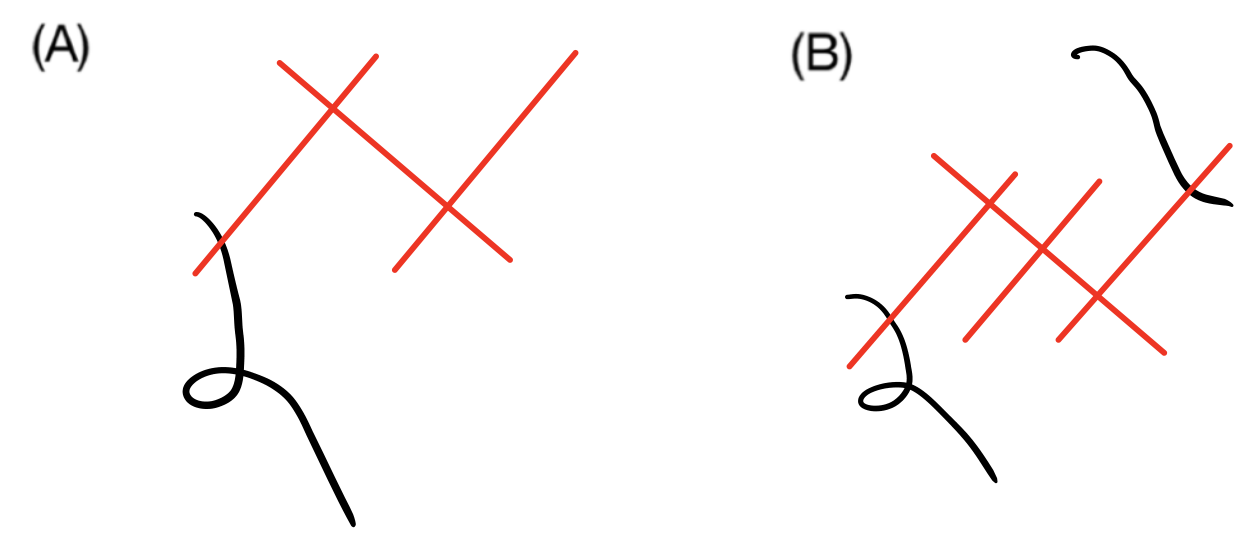
\includegraphics[width=.6\textwidth]{figures/fig-6.6.2.png}
\caption{有理尾和有理桥链.}\label{src:6.6.2}\end{figure}
\begin{corollary}[稳定收缩]\label{src:6.6.3}
设 $(C,\allowbreak p_i)$ 是域 $k$ 上亏格 $g$ 的 $n$-点预稳定曲线, $2g-2+n>0$. 则存在典范态射 $c:C\to\allowbreak C^{\mathrm{st}}$, 称为\newterm{稳定收缩}{stable contraction}, 将所有有理尾和有理桥收缩为点, 使 $(C^{\mathrm{st}},\allowbreak c(p_i))$ 为亏格 $g$ 的 $n$-点稳定曲线, $c_*\mathcal O_C=\mathcal O_{C^{\mathrm{st}}}$, $\mathrm R^1c_*\mathcal O_C=0$. 此外, $c$ 的构造与 $k$ 的域扩张交换.
\end{corollary}
\begin{proof}
令 $E$ 为所有有理尾和有理桥的概形论并, 则 $\mathrm H^0(E,\allowbreak \mathcal O_E)$ 是有限个域的乘积. 反复应用命题~\bookref{6.6.1}, 得到推出图
\[
\begin{tikzcd}
E\arrow[r]\arrow[d]&C\arrow[d,"c"]\\
\Spec\mathrm H^0(E,\mathcal O_E)\arrow[r]\arrow[ur,phantom,"\lrcorner"]&C^{\mathrm{st}},
\end{tikzcd}
\]
满足 $c_*\mathcal O_C=\mathcal O_{C^{\mathrm{st}}}$, $\mathrm R^1c_*\mathcal O_C=0$, 且 $c$ 的构造与域扩张交换. 因为 $(C^{\mathrm{st}},\allowbreak c(p_i))$ 不含有理尾和有理桥, 它稳定 (命题~\bookref{6.3.15}). 另见~\cite[Tag 0E7Q]{SP}.
\end{proof}
\begin{figure}[H]\centering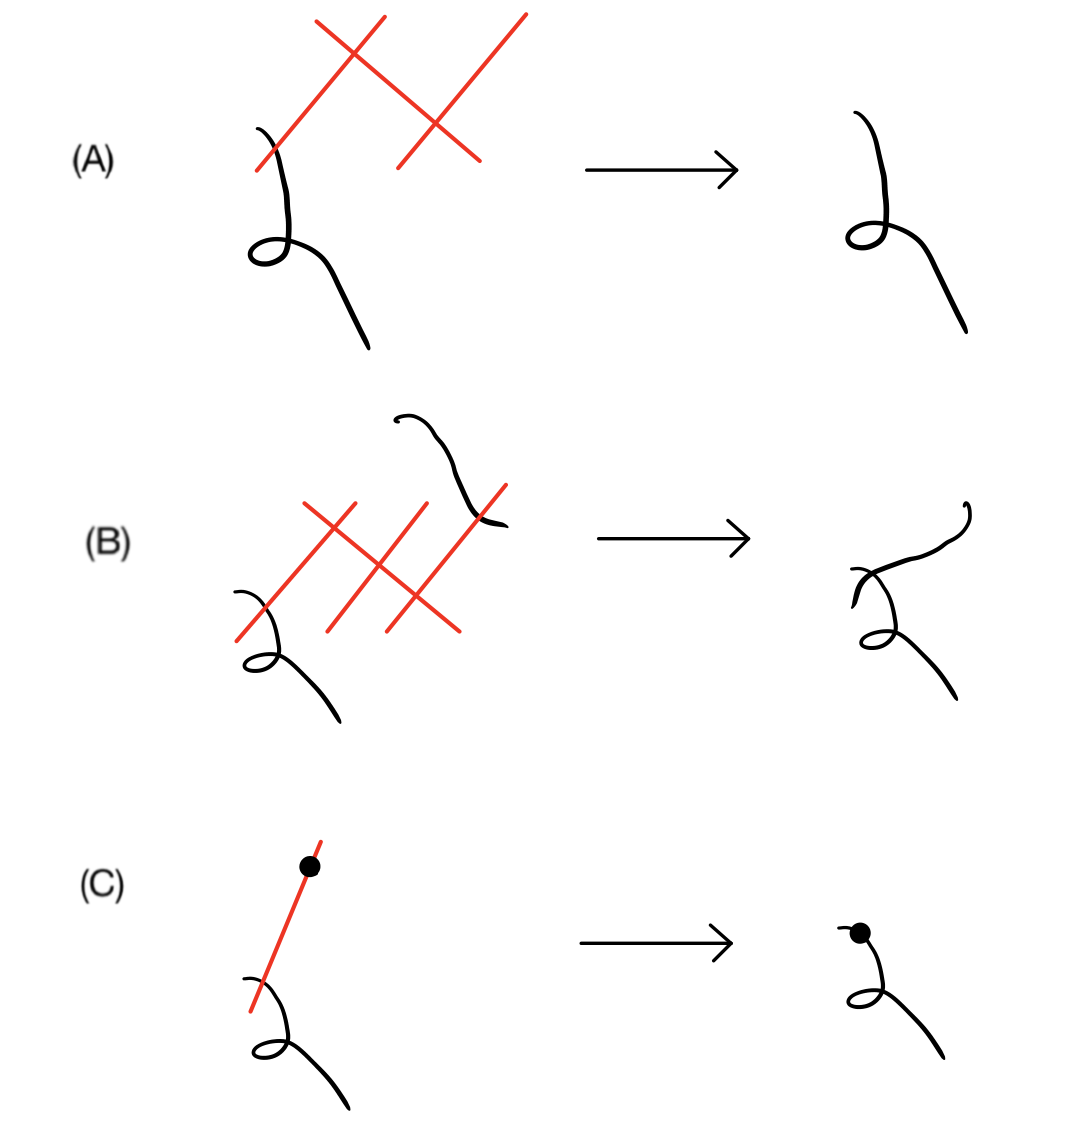
\includegraphics[width=.55\textwidth]{figures/fig-6.6.4.png}
\caption{稳定收缩.}\label{src:6.6.4}\end{figure}
\begin{exercise}\label{src:6.6.5}
设 $(C,\allowbreak p_i)$ 是域 $k$ 上的 $n$-点预稳定曲线.
\begin{enumerate}[(a)]
\item 证明稳定化态射 $c:C\to\allowbreak C^{\mathrm{st}}$ 是满足 $(C^{\mathrm{st}},\allowbreak c(p_i))$ 稳定, $c_*\mathcal O_C=\mathcal O_{C^{\mathrm{st}}}$, $\mathrm R^1c_*\mathcal O_C=0$ 的唯一态射.
\item 若 $(C,\allowbreak p_i)$ 半稳定, $L:=\omega_C(\sum_i p_i)$, 证明 $C^{\mathrm{st}}\cong\operatorname{Proj}\bigoplus_{d\geq0}\mathrm H^0(C,\allowbreak L^{\otimes d})$, 且 $L\cong c^*\omega_{C^{\mathrm{st}}}(\sum_i c(p_i))$.
\end{enumerate}
\end{exercise}
稳定收缩的构造可推广到预稳定曲线族.
\begin{theorem}[预稳定族的稳定收缩]\label{src:6.6.6}
若 $(\mathcal C\to\allowbreak S,\allowbreak \sigma_i)$ 是亏格 $g$ 的 $n$-点预稳定曲线族, $2g-2+n>0$, 则存在唯一的 $S$ 上态射 $c:\mathcal C\to\mathcal C^{\mathrm{st}}$, 使得
\begin{enumerate}[(1)]
\item $(\mathcal C^{\mathrm{st}}\to\allowbreak S,\allowbreak \sigma_i^{\mathrm{st}})$ 是亏格 $g$ 的 $n$-点稳定曲线族, 其中 $\sigma_i^{\mathrm{st}}=c\circ\sigma_i$;
\item $\mathcal O_{\mathcal C^{\mathrm{st}}}=c_*\mathcal O_{\mathcal C}$, $\mathrm R^1c_*\mathcal O_{\mathcal C}=0$;
\item $c:\mathcal C\to\mathcal C^{\mathrm{st}}$ 的构造与基变换 $S'\to\allowbreak S$ 相容;
\item 对每个 $s\in S$, $(\mathcal C_s,\allowbreak \sigma_i(s))\to(\mathcal C_s^{\mathrm{st}},\allowbreak \sigma_i^{\mathrm{st}}(s))$ 是推论~\bookref{6.6.3} 中有理桥和有理尾的稳定收缩.
\end{enumerate}
此外, 若 $(\pi:\mathcal C\to\allowbreak S,\allowbreak \sigma_i)$ 是半稳定族, 则 $\omega_{\mathcal C/S}(\sum_i\sigma_i)$ 是相对丰沛线丛 $L:=\omega_{\mathcal C^{\mathrm{st}}/S}(\sum_i\sigma_i^{\mathrm{st}})$ 的拉回; 特别地, $\mathcal C^{\mathrm{st}}\cong\operatorname{Proj}_S\bigoplus_{d\geq0}\pi_*(L^{\otimes d})$.
\end{theorem}
\begin{proof}
给出从局部到整体的论证. 对任意 $s\in S$, 推论~\bookref{6.6.3} 给出 $\kappa(s)$ 上的稳定收缩 $c_s:\mathcal C_s\to\allowbreak Y_0$, 由习题~\bookref{6.6.5}(a) 满足唯一性. 关键思想如下: 因为 $c_{s,\allowbreak *}\mathcal O_{\mathcal C_s}=\mathcal O_{Y_0}$, $\mathrm R^1c_{s,\allowbreak *}\mathcal O_{\mathcal C_s}=0$, $\mathcal C_s$ 的任意无穷小形变唯一延拓为 $\mathcal C_s\to\allowbreak Y_0$ 的形变 (习题~\bookref{C.2.9}). 置 $S_n=\Spec\mathcal O_{S,\allowbreak s}/\mathfrak m^{n+1}$, 得到 $S_n$ 上相容的态射
\[
\mathcal C\times_S S_n\to Y_n.
\]
Artin 逼近 (\bookref{B.5.18}) 在平展覆盖 $S'\to\allowbreak S$ 后给出态射 $\mathcal C\times_S S'\to\allowbreak Y'$, 由唯一性下降为 $\mathcal C\to\mathcal C^{\mathrm{st}}$.

为使此论证成立, 先用极限方法 (\bookref{B.3} 节) 归结到 $S$ 在 $\mathbb Z$ 上有限型. 如第一段, 找到 $S_n$ 上相容的态射 $\mathcal C\times_S S_n\to\allowbreak Y_n$. 由命题~\bookref{5.5.19}, 中心纤维 $\mathcal C_s$, $Y_0$ 是概形, 故 $\mathcal C\times_S S_n$, $Y_n$ 也是概形. 因为 $\widehat S:=\Spec\widehat{\mathcal O}_{S,\allowbreak s}$ 是 Noether 的, Grothendieck 存在定理 (推论~\bookref{C.5.8}) 给出射影态射 $\widehat Y\to\widehat S$, 延拓 $Y_n\to\allowbreak S_n$. 由平坦性的无穷小判据 (\bookref{A.2.5}), $\widehat Y\to\widehat S$ 平坦. Grothendieck 存在定理的推论 (\bookref{C.5.11}) 给出延拓 $\mathcal C\times_S S_n\to\allowbreak Y_n$ 的 $\widehat S$ 上态射 $\mathcal C\times_S\widehat S\to\widehat Y$. 令 $\widehat\tau_i$ 为复合 $\widehat S\xrightarrow{\sigma_i\times_S\widehat S}\mathcal C\times_S\widehat S\to\widehat Y$, 则 $(\widehat Y\to\widehat S,\allowbreak \widehat\tau_i)$ 是 $n$-点曲线族. 中心纤维 $Y_0$ 稳定, 故稳定性的开放性 (\bookref{6.3.24}) 保证它是稳定曲线族.

因为 $S$ 在 $\mathbb Z$ 上有限型, Artin 逼近 (\bookref{B.5.18}) 给出平展邻域 $(S',\allowbreak s')\to(S,\allowbreak s)$, 稳定曲线族 $(Y'\to\allowbreak S',\allowbreak \tau_i)$ 和 $S'$ 上代数空间的态射 $c':\mathcal C\times_S S'\to\allowbreak Y'$, 在 $s'$ 处的纤维对应于 $\mathcal C_s\to\allowbreak Y_0$. 由习题~\bookref{6.6.8}, 将 $S'$ 换为 $s'$ 的开邻域后, 可假设 $c_*\mathcal O_{\mathcal C\times_S S'}=\mathcal O_{Y'}$, $\mathrm R^1c_*\mathcal O_{\mathcal C\times_S S'}=0$, 且在基变换后仍成立. 一旦建立唯一性, 所需稳定曲线族的存在性便由平展下降得出.

为证唯一性, 设 $(Y\to\allowbreak S,\allowbreak \tau_i)$, $(Y'\to\allowbreak S,\allowbreak \tau'_i)$ 是稳定曲线族, $c:\mathcal C\to\allowbreak Y$, $c':\mathcal C\to\allowbreak Y'$ 是 $S$ 上态射, 并假设有与 $c_s$, $c'_s$ 相容的同构 $\alpha_s:Y_s\xrightarrow{\sim}Y'_s$, 且 $c_{s,\allowbreak *}\mathcal O_{\mathcal C_s}=\mathcal O_{Y_s}$, $\mathrm R^1c_{s,\allowbreak *}\mathcal O_{\mathcal C_s}=0$. 需证存在 $s$ 的开邻域 $U\subseteq S$ 和延拓 $\alpha_s$ 的同构 $\alpha:Y_U\to\allowbreak Y'_U$, 与 $c_U$, $c'_U$ 相容. 由极限方法 (\bookref{B.3} 节), 可假设 $S=\Spec A$, $A$ 为 Noether 局部环. 令 $Y''$ 为 $\mathcal C\to\allowbreak Y\times_S Y'$ 的概形论像, 只需证投影 $Y''\to\allowbreak Y$, $Y''\to\allowbreak Y'$ 为同构. 因为概形论像与平坦基变换交换, 还可假设 $A$ 完备. 由习题~\bookref{C.2.9}, 基变换到 $\Spec A/\mathfrak m^{n+1}$ 后的限制 $Y''_n\to\allowbreak Y_n$, $Y''_n\to\allowbreak Y'_n$ 都是同构. Grothendieck 存在定理的推论 (\bookref{C.5.11}) 给出所需同构 $Y\to\allowbreak Y'$. 另见~\cite[Tag 0E8A]{SP}.

若 $(\mathcal C\to\allowbreak S,\allowbreak \sigma_i)$ 是半稳定曲线族, 则断言自然映射 $c^*\omega_{\mathcal C^{\mathrm{st}}/S}\to\omega_{\mathcal C/S}$ 是同构. 相对对偶化层是线丛, 因而只需证此映射满射. 因为相对对偶化层和该映射的余核与基变换相容, 由 Nakayama 引理, 只需在 $S$ 为域的谱时证明断言, 这正是习题~\bookref{6.6.5}(b). 由投影公式, $\omega_{\mathcal C^{\mathrm{st}}/S}\cong c_*c^*\omega_{\mathcal C^{\mathrm{st}}/S}$, 从而复合 $\omega_{\mathcal C^{\mathrm{st}}/S}\cong c_*c^*\omega_{\mathcal C^{\mathrm{st}}/S}\to\allowbreak c_*\omega_{\mathcal C/S}$ 是同构. 因此
\[
\omega_{\mathcal C^{\mathrm{st}}/S}\Bigl(\sum_i\sigma_i^{\mathrm{st}}\Bigr)
\cong c_*\Bigl(\omega_{\mathcal C/S}\Bigl(\sum_i\sigma_i\Bigr)\Bigr),
\]
这由 $\omega_{\mathcal C^{\mathrm{st}}/S}$ 相对甚丰沛 (命题~\bookref{6.3.22}) 推出所述结论. 或者可通过证明自然映射 $\pi_*(L^{\otimes2})\otimes\pi_*(L^{\otimes d})\to\pi_*(L^{\otimes(d+2)})$ 对 $d\geq4$ 满射, 在整体上明确构造稳定收缩. 从而 $\bigoplus_{d\geq0}\pi_*(L^{\otimes4d})$ 是有限型 $\mathcal O_S$-代数, 可定义 $\mathcal C^{\mathrm{st}}:=\operatorname{Proj}_S\bigoplus_{d\geq0}\pi_*(L^{\otimes4d})$. 因为对所有 $d\geq0$, 推前 $\pi_*(L^{\otimes4d})$ 是向量丛, 其构造与基变换交换 (命题~\bookref{6.3.23}), $\mathcal C\to\mathcal C^{\mathrm{st}}$ 良定义, $\mathcal C^{\mathrm{st}}\to\allowbreak S$ 是稳定曲线族. 见~\cite[命题 2.1]{Knu83a} 和~\cite[命题 10.6.7]{ACG11}.
\end{proof}
\begin{corollary}[稳定收缩态射]\label{src:6.6.7}
存在代数叠的态射
\[
\mathcal M_{g,n}^{\mathrm{pre}}\to\overline{\mathcal M}_{g,n},\qquad
(C,p_i)\mapsto(C^{\mathrm{st}},c(p_i)),
\]
在开子叠 $\overline{\mathcal M}_{g,\allowbreak n}\subseteq\mathcal M_{g,\allowbreak n}^{\mathrm{pre}}$ 上为恒等.
\end{corollary}
\newpage
\begin{exercise}[细节]\label{src:6.6.8}
设 $f:X\to\allowbreak Y$ 是 Noether 概形 $S$ 上曲线族的态射. 假设对某点 $s\in S$, 态射 $f_s:X_s\to\allowbreak Y_s$ 满足 $f_{s,\allowbreak *}\mathcal O_{X_s}=\mathcal O_{Y_s}$, $\mathrm R^1f_{s,\allowbreak *}\mathcal O_{X_s}=0$. 证明将 $S$ 换为 $s$ 的开邻域后, 有 $f_*\mathcal O_X=\mathcal O_Y$, $\mathrm R^1f_*\mathcal O_X=0$, 且沿态射 $S'\to\allowbreak S$ 基变换后仍成立. 另见~\cite[Tag 0E88]{SP}.
\end{exercise}
\subsection{\texorpdfstring{遗忘态射与 $\overline{\mathcal M}_{g,\allowbreak n}$ 的泛族}{遗忘态射与 稳定曲线模叠 的泛族}}\label{src:6.6.2-subsection}
给出稳定收缩态射 (\bookref{6.6.7}) 的两个推论: 存在映射 $\overline{\mathcal M}_{g,\allowbreak n+1}\to\overline{\mathcal M}_{g,\allowbreak n}$, 它是在遗忘最后一个标记点之后的稳定收缩, 且可认同为泛族.
\begin{figure}[H]\centering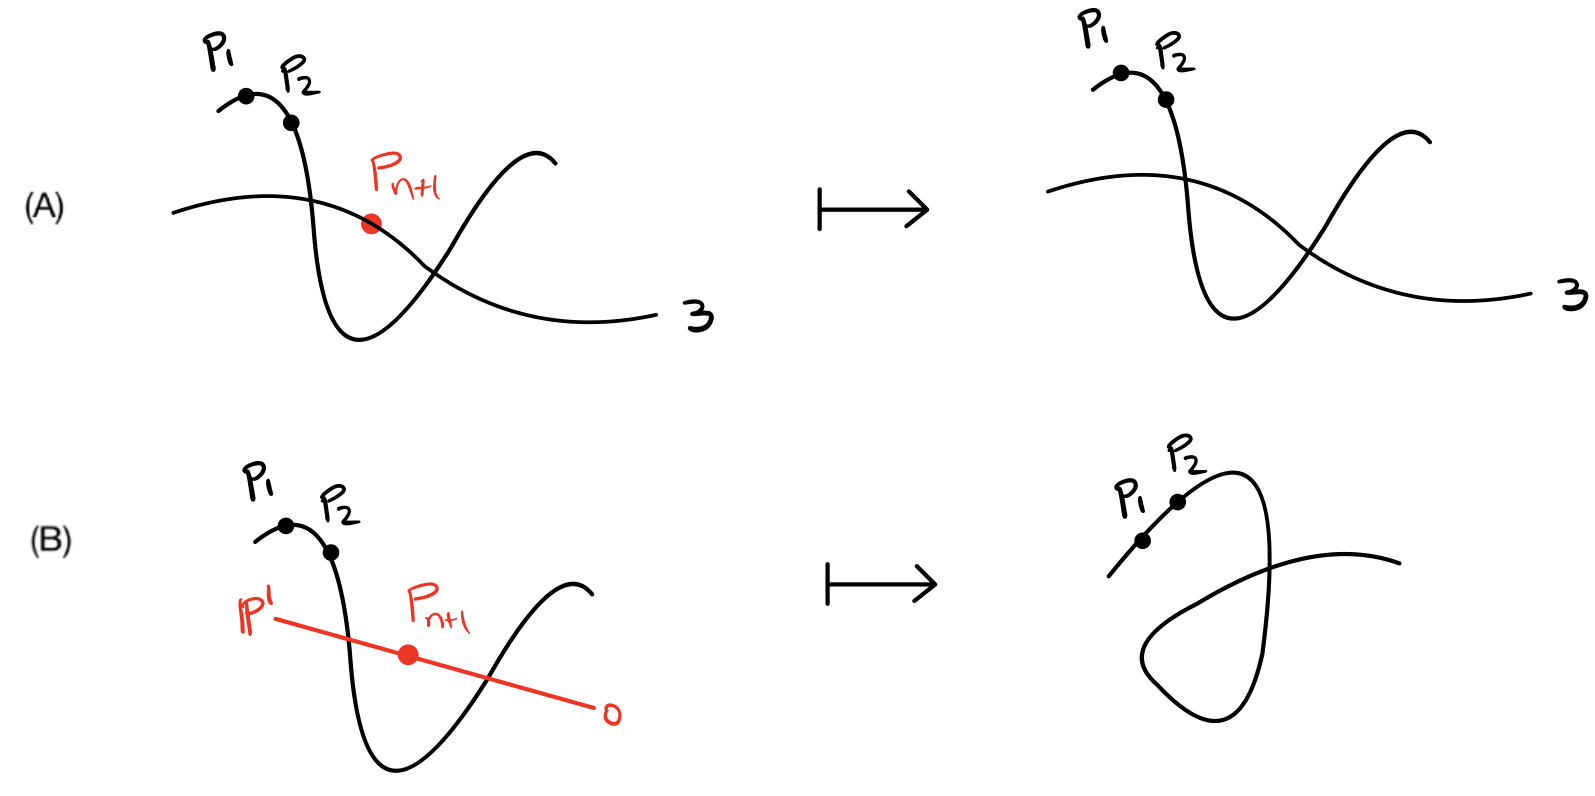
\includegraphics[width=.7\textwidth]{figures/fig-6.6.9.png}
\caption{(A) 中只需遗忘第 $n+1$ 个点. (B) 中若遗忘 $p_{n+1}$, 曲线不再稳定, 必须收缩有理桥.}\label{src:6.6.9}\end{figure}
\begin{proposition}[遗忘态射]\label{src:6.6.10}
存在代数叠的态射
\[
\overline{\mathcal M}_{g,n+1}\to\overline{\mathcal M}_{g,n},\qquad
(C,p_1,\ldots,p_{n+1})\mapsto(C^{\mathrm{st}},c(p_1),\ldots,c(p_n)),
\]
其中 $c:C\to\allowbreak C^{\mathrm{st}}$ 是 $(C,\allowbreak p_1,\allowbreak \ldots,\allowbreak p_n)$ 的稳定收缩.
\end{proposition}
\begin{proof}
所需态射构造为复合
\[
\overline{\mathcal M}_{g,n+1}\to\mathcal M_{g,n}^{\mathrm{pre}}\to\overline{\mathcal M}_{g,n},
\]
其中第一箭头将 $(n+1)$-点稳定族 $(\mathcal C\to\allowbreak S,\allowbreak \sigma_1,\allowbreak \ldots,\allowbreak \sigma_{n+1})$ 映为 $n$-点预稳定族 $(\mathcal C\to\allowbreak S,\allowbreak \sigma_1,\allowbreak \ldots,\allowbreak \sigma_n)$, 第二箭头是稳定收缩态射 (\bookref{6.6.7}).
\end{proof}
由广义 $2$-Yoneda 引理 (\bookref{4.1.27}), 恒等态射 $\overline{\mathcal M}_{g,\allowbreak n}\to\overline{\mathcal M}_{g,\allowbreak n}$ 对应于代数叠 $\overline{\mathcal M}_{g,\allowbreak n}$ 上的一个 $\overline{\mathcal M}_{g,\allowbreak n}$ 对象, 后者通过下降对应于 $n$-点稳定曲线族
\[
(\mathcal U_{g,n}\to\overline{\mathcal M}_{g,n},\sigma_1^{\mathrm{univ}},\ldots,\sigma_n^{\mathrm{univ}}),
\]
称为泛族. $\mathcal U_{g,\allowbreak n}$ 在概形 $S$ 上的对象是 $n$-点稳定曲线族 $(\mathcal C\to\allowbreak S,\allowbreak \sigma_i)$, 配备额外截面 $\tau:S\to\mathcal C$ (它可落入 $\mathcal C\to\allowbreak S$ 的结点轨迹, 也可与 $\sigma_i$ 非平凡相交). 给定 $n$-点稳定曲线族 $(\mathcal C\to\allowbreak S,\allowbreak \sigma_i)$, 存在在唯一同构意义下唯一的态射 $S\to\overline{\mathcal M}_{g,\allowbreak n}$ 及 Cartesian 图
\[
\begin{tikzcd}
\mathcal C\arrow[r]\arrow[d,shift right=1ex]&\mathcal U_{g,n}\arrow[d,shift right=1ex]\\
S\arrow[r]\arrow[u,shift right=1ex,"\sigma_i"]&\overline{\mathcal M}_{g,n}\arrow[u,shift right=1ex,"\sigma_i^{\mathrm{univ}}"'].
\end{tikzcd}
\]
另一方面, 有遗忘态射 (\bookref{6.6.10}) 和代数叠的态射 $\overline{\mathcal M}_{g,\allowbreak n+1}\to\mathcal U_{g,\allowbreak n}$, 将 $(n+1)$-点稳定族 $(\mathcal C\to\allowbreak S,\allowbreak \sigma_i)$ 映为 $(\mathcal C^{\mathrm{st}},\allowbreak \sigma_1^{\mathrm{st}},\allowbreak \ldots,\allowbreak \sigma_n^{\mathrm{st}},\allowbreak c\circ\sigma_{n+1})$, 其中 $c:\mathcal C\to\mathcal C^{\mathrm{st}}$ 是预稳定族 $(\mathcal C,\allowbreak \sigma_1,\allowbreak \ldots,\allowbreak \sigma_n)$ 的稳定收缩 (\bookref{6.6.6}). 得到交换图
\[
\begin{tikzcd}
\overline{\mathcal M}_{g,n+1}\arrow[rr]\arrow[dr]&&\mathcal U_{g,n}\arrow[dl]\\
&\overline{\mathcal M}_{g,n}.&
\end{tikzcd}
\]
\begin{figure}[H]\centering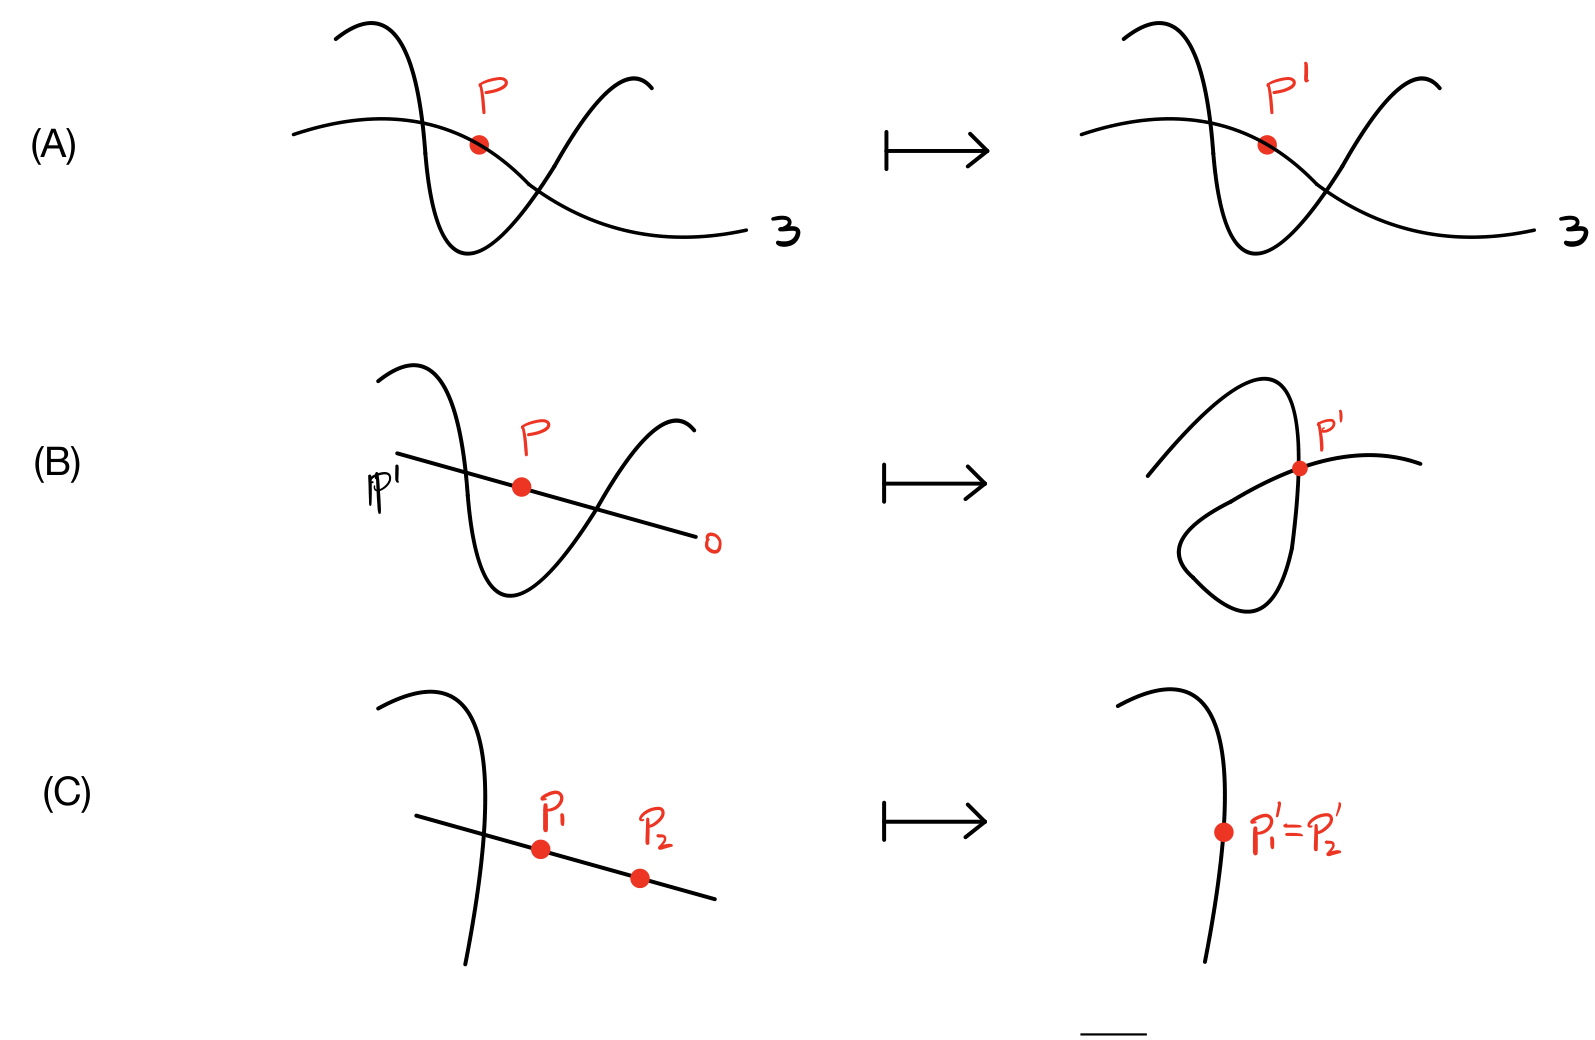
\includegraphics[width=.65\textwidth]{figures/fig-6.6.11.png}
\caption{映射 $\overline{\mathcal M}_{g,\allowbreak n}\to\mathcal U_{g,\allowbreak n}$ 的例子.}\label{src:6.6.11}\end{figure}
\begin{proposition}\label{src:6.6.12}
态射 $\overline{\mathcal M}_{g,\allowbreak n+1}\to\mathcal U_{g,\allowbreak n}$ 是 $\overline{\mathcal M}_{g,\allowbreak n}$ 上的同构. 换言之, 遗忘态射 $\overline{\mathcal M}_{g,\allowbreak n+1}\to\overline{\mathcal M}_{g,\allowbreak n}$ 是泛族.
\end{proposition}
\begin{proof}
由稳定约化 (\bookref{6.5.1}), 两个叠 $\overline{\mathcal M}_{g,\allowbreak n+1}$ 和 $\mathcal U_{g,\allowbreak n}$ 在 $\overline{\mathcal M}_{g,\allowbreak n}$ 上均固有且可表. 因而 $\overline{\mathcal M}_{g,\allowbreak n+1}\to\mathcal U_{g,\allowbreak n}$ 固有且可表. 对每个代数闭域 $k$, 同构类上的诱导映射 $\overline{\mathcal M}_{g,\allowbreak n+1}(k)/{\sim}\to\mathcal U_{g,\allowbreak n}(k)/{\sim}$ 是双射. 故该态射固有拟有限, 因而有限. 另一方面, 它在参数化 $(C,\allowbreak p_1,\allowbreak \ldots,\allowbreak p_n)$ 不含有理桥的带标记曲线 $(C,\allowbreak p_1,\allowbreak \ldots,\allowbreak p_{n+1})$ 的开子叠, 与参数化 $p_{n+1}\in C$ 为不与 $p_1,\allowbreak \ldots,\allowbreak p_n$ 重合的光滑点的开子叠之间诱导同构, 故双有理. 由定理~\bookref{6.4.16}, $\overline{\mathcal M}_{g,\allowbreak n+1}$ 光滑. 因为 $\mathcal U_{g,\allowbreak n}\to\overline{\mathcal M}_{g,\allowbreak n}$ 的纤维是 Cohen--Macaulay 的, 且基底光滑, $\mathcal U_{g,\allowbreak n}$ 是 Cohen--Macaulay 的. 此叠在 $p_{n+1}\in C$ 为光滑点的开轨迹上正则, 该轨迹的补集的余维为 $2$, 故 Serre 正规性判据保证 $\mathcal U_{g,\allowbreak n}$ 正规. 正规 Deligne--Mumford 叠之间的有限双有理态射必为同构.
\end{proof}
\begin{remark}\label{src:6.6.13}
还可显式构造逆态射 $\mathcal U_{g,\allowbreak n}\to\overline{\mathcal M}_{g,\allowbreak n+1}$. 设 $(\mathcal C\to\allowbreak S,\allowbreak \sigma_i)$ 为 $n$-点稳定曲线族, $\tau:S\to\mathcal C$ 是由理想层 $\mathcal I_\tau$ 定义的额外截面. 由
\[
0\to\mathcal O_{\mathcal C}\xrightarrow{(\alpha,\beta)}\mathcal I_\tau^\vee\oplus\mathcal O_{\mathcal C}(\sigma_1+\cdots+\sigma_n)\to\mathcal K\to0
\]
定义凝聚 $\mathcal O_{\mathcal C}$-模 $\mathcal K$, 其中 $\alpha$ 是包含 $\mathcal I_\tau\hookrightarrow\mathcal O_{\mathcal C}$ 的对偶, $\beta$ 为自然包含. 定义
\[
\widetilde{\mathcal C}=\operatorname{Proj}_S\operatorname{Sym}\mathcal K\to\mathcal C.
\]
经过一些工作可证 $\tau^*(\mathcal I_\tau^\vee/\mathcal O_{\mathcal C})$ 为线丛~\cite[引理 2.2]{Knu83a}. 满射 $\tau^*\mathcal K\to\tau^*(\mathcal K/\mathcal O_{\mathcal C})\cong\tau^*(\mathcal I_\tau^\vee/\mathcal O_{\mathcal C})$ 定义截面 $\widetilde\tau:S\to\widetilde{\mathcal C}$. 单射 $\mathcal I_\tau^\vee\to\mathcal K$ 的余核可认同为 $\mathcal O_{\mathcal C}(\sigma_1+\cdots+\sigma_n)|_{\bigcup_i\sigma_i}$, 满射 $\sigma_i^*\mathcal K\to\sigma_i^*\mathcal O_{\mathcal C}(\sigma_1+\cdots+\sigma_n)$ 定义截面 $\widetilde\sigma_i:S\to\widetilde{\mathcal C}$. 可检验 $(\widetilde{\mathcal C}\to\allowbreak S,\allowbreak \widetilde\sigma_1,\allowbreak \ldots,\allowbreak \widetilde\sigma_n,\allowbreak \widetilde\tau)$ 是 $(n+1)$-点稳定曲线族, $c:\widetilde{\mathcal C}\to\mathcal C$ 是 $n$-点预稳定族 $(\widetilde{\mathcal C},\allowbreak \widetilde\sigma_1,\allowbreak \ldots,\allowbreak \widetilde\sigma_n)$ 的稳定收缩, 且 $\sigma_i=c\circ\widetilde\sigma_i$, $\tau=c\circ\widetilde\tau$. 许多情形中, $\widetilde{\mathcal C}\to\mathcal C$ 可更直接地构造为爆破: 例如, 若 $\mathcal C\to\allowbreak S$ 是离散赋值环谱上的一般光滑稳定曲线族, $\mathcal C$ 正则, $\tau:S\to\mathcal C$ 为截面且 $\tau(0)\in\mathcal C_0$ 是结点, 则 $\widetilde{\mathcal C}\to\mathcal C$ 就是在 $\tau(0)$ 处的爆破, $\widetilde\tau$ 是 $\tau$ 的严格变换. 见~\cite[定理 2.4]{Knu83a} 和~\cite[\S X.8]{ACG11}.
\end{remark}
\subsection{粘合态射}\label{src:6.6.3-subsection}
证明曲线族的截面可粘为结点族 (命题~\bookref{6.6.15}) 后, 我们说明存在良定义的有限态射 $\overline{\mathcal M}_{i,\allowbreak k}\times\overline{\mathcal M}_{g-i,\allowbreak n-k+2}\to\overline{\mathcal M}_{g,\allowbreak n}$ 和 $\overline{\mathcal M}_{g-1,\allowbreak n+2}\to\overline{\mathcal M}_{g,\allowbreak n}$ (推论~\bookref{6.6.16}), 称为\newterm{粘合态射}{gluing morphism} (有时也称 clutching morphism).
\begin{figure}[H]\centering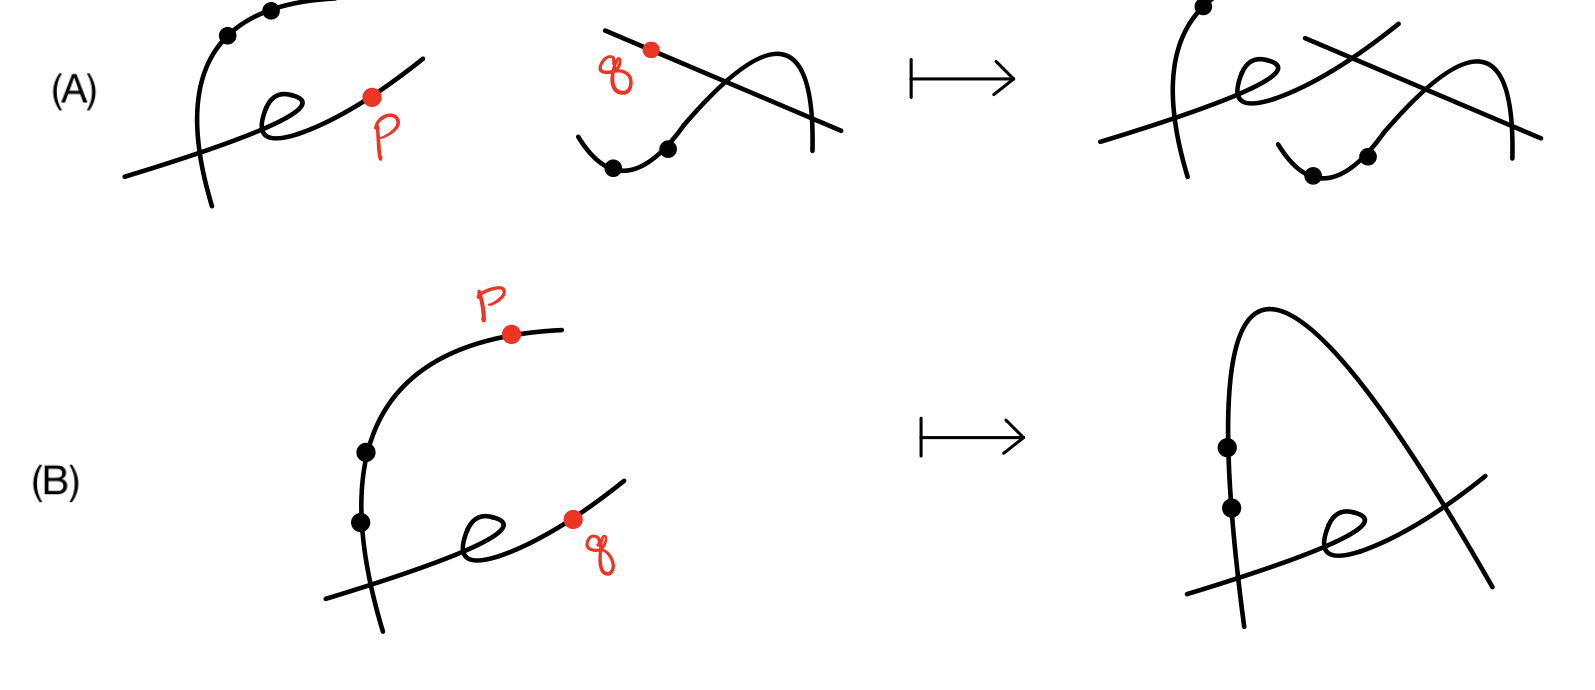
\includegraphics[width=.7\textwidth]{figures/fig-6.6.14.png}
\caption{标记点 $p$, $q$ 的结点粘合.}\label{src:6.6.14}\end{figure}
\begin{proposition}[沿截面粘合族]\label{src:6.6.15}
设 $(\mathcal C\to\allowbreak S,\allowbreak \sigma,\allowbreak \tau)$ 是概形 $S$ 上的 $2$-点射影曲线族 (可不连通), 使每个 $s\in S$ 的 $\sigma(s)$, $\tau(s)$ 为 $\mathcal C_s$ 的互异光滑点. 则存在 $S$ 上概形的典范有限态射 $g:\mathcal C\to\mathcal C'$, 使得
\begin{enumerate}[(1)]
\item $\mathcal C'\to\allowbreak S$ 是曲线族, 带截面 $\nu:S\to\mathcal C'$, 满足 $\nu=g\circ\sigma=g\circ\tau$, 且每个 $s\in S$ 的 $\nu(s)\in\mathcal C_s$ 是结点;
\item $g$ 限制为同构 $\mathcal C\setminus(\sigma(S)\cup\tau(S))\xrightarrow{\sim}\mathcal C'\setminus\nu(S)$, 拓扑空间 $|\mathcal C'|$ 可认同为 $|\mathcal C|$ 对等价关系 $\sigma(s)\sim\tau(s)$ ($s\in S$) 的商;
\item $\mathcal C'$ 可认同为 $\sigma\amalg\tau:S\amalg S\to\mathcal C$ 与投影 $S\amalg S\to\allowbreak S$ 的 Ferrand 推出 (\bookref{B.4.1}); 特别地, 对每个开集 $U\subseteq\mathcal C'$,
\[
\Gamma(U,\mathcal C')=\{f\in\Gamma(g^{-1}(U),\mathcal C)\mid\sigma^*f=\tau^*f\};
\]
\item 此构造与基变换 $T\to\allowbreak S$ 相容.
\end{enumerate}
\end{proposition}
\begin{proof}
因为 $\mathcal C\to\allowbreak S$ 射影, 纤维 $\mathcal C_s$ 的任意两点包含在 $\mathcal C$ 的一个仿射开子概形中. 因而 Ferrand 推出 (\bookref{B.4.1})
\[
\begin{tikzcd}
S\amalg S\arrow[r,"\sigma\amalg\tau"]\arrow[d]&\mathcal C\arrow[d]\\
S\arrow[r,"\nu"']\arrow[ur,phantom,"\lrcorner"]&\mathcal C'
\end{tikzcd}
\]
作为概形 $\mathcal C'$ 存在. 由推出的泛性质, 有自然映射 $\mathcal C'\to\allowbreak S$. 因为 $S\amalg S\to\allowbreak S$ 有限, $\mathcal C\to\mathcal C'$ 也有限. 因为 $S\amalg S\to\allowbreak S$ 平坦, 由推出的性质 (\bookref{B.4.8}(4)), 构造与任意基变换相容. 这给出 (2)--(4).

为证 (1), 先注意 $\mathcal C\to\mathcal C'$ 有限, 故 $\mathcal C'\to\allowbreak S$ 固有. 由光滑态射的局部结构 (\bookref{A.3.4}), 对每个 $s\in S$, 存在仿射开邻域 $\Spec A\subseteq S$ 以及 $\sigma(s)$, $\tau(s)$ 的平展邻域 $\mathcal C\to\Spec A[x]$, $\mathcal C\to\Spec A[y]$. 由推出的性质 (\bookref{B.4.8}(3)), $\mathcal C'$ 在 $\nu(s)$ 处有与如下推出同构的平展邻域:
\[
\begin{tikzcd}
\Spec(A\times A)\arrow[r,"0\amalg0"]\arrow[d]&\Spec(A[x]\times A[y])\arrow[d]\\
\Spec A\arrow[r]\arrow[ur,phantom,"\lrcorner"]&\Spec A[x,y]/(xy).
\end{tikzcd}
\]
所以 $\mathcal C'\to\allowbreak S$ 平坦, $\nu(s)\in\mathcal C_s$ 是结点.

若 $\omega_{\mathcal C/S}(\sigma+\tau)$ 相对甚丰沛 (应用于稳定曲线时即如此), 也可用整体 $\operatorname{Proj}$ 构造 $\mathcal C'$. 有良定义的态射 $q_\sigma:\omega_{\mathcal C/S}(\sigma+\tau)\to\mathcal O_{\sigma(S)}$ 和 $q_\tau:\omega_{\mathcal C/S}(\sigma+\tau)\to\mathcal O_{\tau(S)}$. 定义 $\mathcal C':=\operatorname{Proj}_S\bigoplus_{d\geq0}\mathcal A_d$, 其中 $\mathcal A_d$ 为纤维积
\[
\begin{tikzcd}[column sep=small]
\mathcal A_d\arrow[r]\arrow[d]&\mathcal O_S\arrow[d]\\
\pi_*(\omega_{\mathcal C/S}(\sigma+\tau)^{\otimes d})\times\pi_*(\omega_{\mathcal C/S}(\sigma+\tau)^{\otimes d})\arrow[r,"\pi_*(q_\sigma^{\otimes d})\times\pi_*(q_\tau^{\otimes d})"']&\mathcal O_S\times\mathcal O_S,
\end{tikzcd}
\]
$\pi:\mathcal C\to\allowbreak S$ 是结构态射. 基本上用同一论证可验证 $\mathcal C'\to\allowbreak S$ 满足所需性质. 见~\cite[定理 3.4]{Knu83a} 和~\cite[\S X.7]{ACG11}.
\end{proof}
\begin{corollary}[粘合态射]\label{src:6.6.16}
假设 $2g-2+n>0$.
\begin{enumerate}[(1)]
\item 若 $2g_1-2+n_1>0$, 置 $g_2=g-g_1$, $n_2=n-n_1+2$, 则存在代数叠的有限态射
\[
\begin{aligned}
\overline{\mathcal M}_{g_1,n_1}\times\overline{\mathcal M}_{g_2,n_2}&\to\overline{\mathcal M}_{g,n},\\
((C,p_i),(D,q_i))&\mapsto(C\amalg_{p_{n_1}\sim q_{n_2}}D,p_1,\ldots,p_{n_1-1},q_1,\ldots,q_{n_2-1}).
\end{aligned}
\]
\item 若 $g\geq1$, 则存在代数叠的有限态射
\[
\overline{\mathcal M}_{g-1,n+2}\to\overline{\mathcal M}_{g,n},\qquad
(C,p_i)\mapsto(C/_{p_{n+1}\sim p_{n+2}},p_1,\ldots,p_{n-2}).
\]
\end{enumerate}
\end{corollary}
\begin{proof}
两种情形下, 沿截面粘合族 (\bookref{6.6.15}) 直接给出到 $\mathcal M_{g,\allowbreak n}^{\mathrm{pre}}$ 的代数叠态射. 稳定性可在几何纤维上检验, 只需证结点粘合 $C\amalg_{p_{n_1}\sim q_{n_2}}D$ 和 $C/_{p_{n+1}\sim p_{n+2}}$ 稳定. 由带标记正规化可判定稳定性 (习题~\bookref{6.3.7}), 故这显然成立. 两个映射都是固有 Deligne--Mumford 叠之间的拟有限可表态射, 因而有限.
\end{proof}
更一般地, 对有限指标集 $I$, 可定义亏格 $g$ 的 $I$-点稳定曲线, 记此类曲线的叠为 $\overline{\mathcal M}_{g,\allowbreak I}$. 双射 $I\cong\{1,\allowbreak \ldots,\allowbreak n\}$ 诱导同构 $\overline{\mathcal M}_{g,\allowbreak I}\cong\overline{\mathcal M}_{g,\allowbreak n}$. 推论~\bookref{6.6.16} 自然推广为有限态射
\[
\overline{\mathcal M}_{g_1,I_1}\times\overline{\mathcal M}_{g_2,I_2}\to\overline{\mathcal M}_{g_1+g_2,(I_1\cup I_2)\setminus\{i_1,i_2\}},\qquad
\overline{\mathcal M}_{g-1,J}\to\overline{\mathcal M}_{g,J\setminus\{j_1,j_2\}},
\]
分别粘合标记点 $i_1\in I_1$, $i_2\in I_2$, 或 $j_1,\allowbreak j_2\in J$, 并要求满足各叠非空的数值条件.
\subsection{边界除子}\label{src:6.6.4-subsection}
定义 $\overline{\mathcal M}_{g,\allowbreak n}$ 的边界除子 $\delta_{i,\allowbreak I}$, 并证明总边界除子 $\delta$ 是正规交叉除子 (命题~\bookref{6.6.19}). $\overline{\mathcal M}_{g,\allowbreak n}$ 上的线丛将在~\bookref{6.10} 节讨论.
\begin{definition}[边界除子]\label{src:6.6.17}
设 $2g-2+n>0$. 令 $0\leq i\leq g$ 为整数, $I\subseteq\{1,\allowbreak \ldots,\allowbreak n\}$ 为子集, 满足 $1-2i<|I|<2(g-i)+n-1>0$ (保证 $\overline{\mathcal M}_{i,\allowbreak I\cup\{p\}}$ 与 $\overline{\mathcal M}_{g-i,\allowbreak I^c\cup\{q\}}$ 都非空). \newterm{边界除子}{boundary divisor} 定义为 $\overline{\mathcal M}_{g,\allowbreak n}$ 的闭子叠
\[
\begin{aligned}
\delta_{i,I}&=\operatorname{im}\bigl(\overline{\mathcal M}_{i,I\cup\{p\}}\times\overline{\mathcal M}_{g-i,I^c\cup\{q\}}\to\overline{\mathcal M}_{g,I\cup I^c}\cong\overline{\mathcal M}_{g,n}\bigr),\\
\delta_0&=\operatorname{im}\bigl(\overline{\mathcal M}_{g-1,n+2}\to\overline{\mathcal M}_{g,n}\bigr),\\
\delta&=\delta_0\cup\bigcup_{i,I}\delta_{i,I},
\end{aligned}
\]
约定 $g=0$ 时 $\delta_0$ 为空.
\end{definition}
注意 $\delta_{i,\allowbreak I}=\delta_{g-i,\allowbreak I^c}$. 若 $n=0$, 则 $\delta=\delta_0\cup\cdots\cup\delta_{\lfloor g/2\rfloor}$. 若 $g=0$, 则 $\delta$ 是大小 $2\leq|I|\leq n-2$ 的子集 $I$ 对应的 $\delta_I$ 的并.
\begin{figure}[H]\centering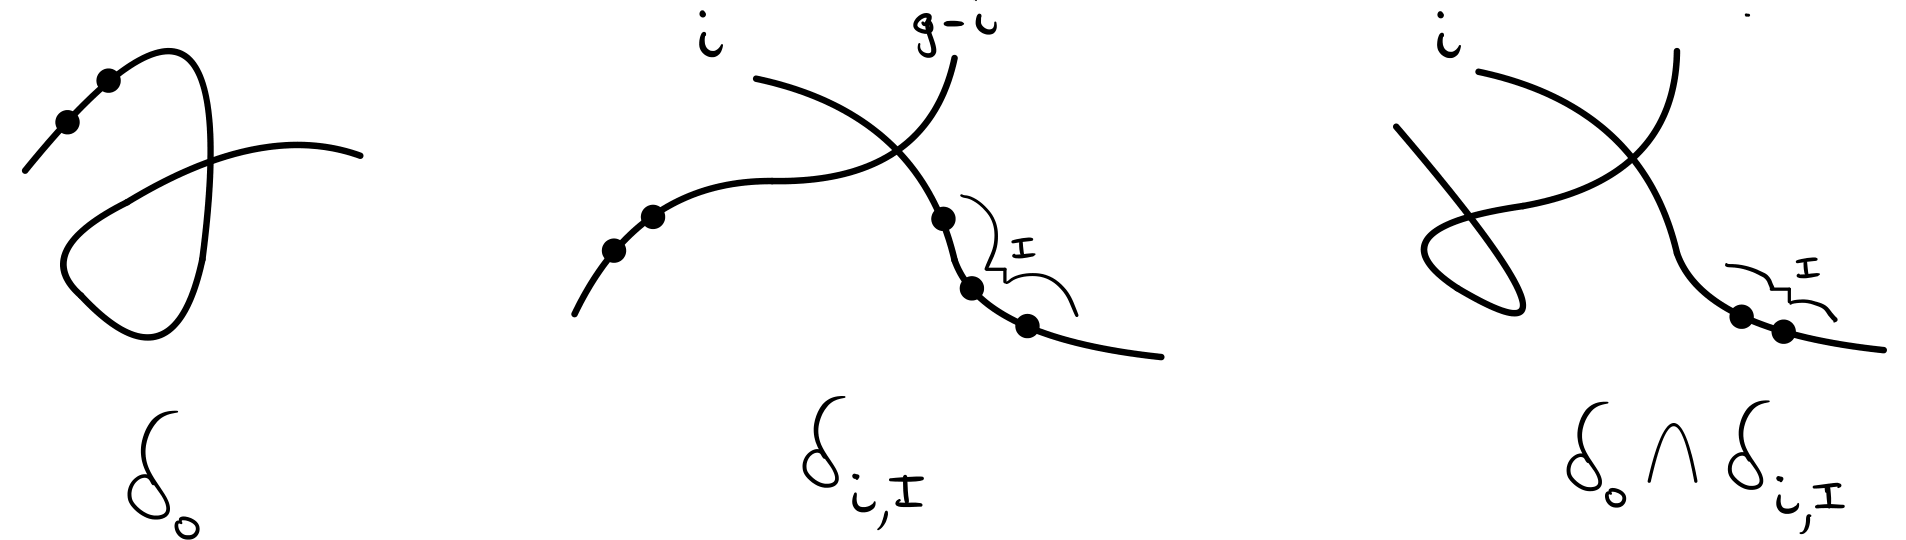
\includegraphics[width=.85\textwidth]{figures/fig-6.6.18.png}
\caption{边界中的稳定曲线的例子.}\label{src:6.6.18}\end{figure}
Deligne--Mumford 叠的闭子叠 $\mathcal Z\subseteq\mathcal X$ 称为有效 Cartier 除子 (分别地, 正规交叉除子), 若有平展展现 $U\to\mathcal X$, 使 $\mathcal Z\times_{\mathcal X}U\subseteq U$ 是有效 Cartier 除子 (分别地, 正规交叉除子). 回顾正则概形的有效 Cartier 除子 $U\subseteq X$ 具有正规交叉, 是指对每个 $u\in U$,
\[
\widehat{\mathcal O}_{U,u}\cong\widehat{\mathcal O}_{X,x}/(f_1\cdots f_k),
\]
其中 $f_1,\allowbreak \ldots,\allowbreak f_k\in\widehat{\mathcal O}_{X,\allowbreak x}$ 可延拓为正则参数系 $f_1,\allowbreak \ldots,\allowbreak f_n$.
\begin{proposition}\label{src:6.6.19}
在域 $k$ 上, $\delta\subseteq\overline{\mathcal M}_{g,\allowbreak n}$ 是正规交叉除子.
\end{proposition}
\begin{proof}
简单的维数计算表明 $\delta$ 纯维, 维数为 $3g-2+n$. 为证正规交叉, 可假设 $k$ 代数闭. 设 $(C,\allowbreak p_i)\in\overline{\mathcal M}_{g,\allowbreak n}$ 是结点为 $q_1,\allowbreak \ldots,\allowbreak q_s\in C$ 的稳定曲线, $(U,\allowbreak u)\to(\overline{\mathcal M}_{g,\allowbreak n},\allowbreak [C,\allowbreak p_i])$ 是平展邻域, $U$ 为概形. 由从局部到整体的形变正合列 (\bookref{6.3.28}), 有一阶形变空间的满射
\begin{equation}\label{src:6.6.20}
\operatorname{Def}(C,p_i)\to\bigoplus_j\operatorname{Def}(\widehat{\mathcal O}_{C,q_j}),
\end{equation}
其中 $\operatorname{Def}(\widehat{\mathcal O}_{C,\allowbreak q_j})\cong k$.

令 $\operatorname{Art}_k$ 为剩余域为 $k$ 的局部 Artin $k$-代数范畴. 定义函子 $F,\allowbreak G_j:\operatorname{Art}_k\to\Sets$: $F(A)$ 为 $(\mathcal C\to\Spec A,\allowbreak \sigma_i,\allowbreak \alpha)$ 的同构类集合, 其中 $(\mathcal C\to\Spec A,\allowbreak \sigma_i)$ 是 $n$-点稳定曲线族, $\alpha:(C,\allowbreak p_i)\xrightarrow{\sim}(\mathcal C\times_A k,\allowbreak \sigma_i\times_A k)$ 为同构; $G_j(A)$ 为 $(B,\allowbreak \beta)$ 的同构类集合, 其中 $B$ 是平坦 $A$-代数, $\beta:\widehat{\mathcal O}_{C,\allowbreak q_j}\xrightarrow{\sim}B\otimes_A A/\mathfrak m_A$ 为同构. 映射 $\Spec\widehat{\mathcal O}_{U,\allowbreak u}\to\overline{\mathcal M}_{g,\allowbreak n}$ 诱导 $F$ 在 $k[[x_1,\allowbreak \ldots,\allowbreak x_{3g-3+n}]]$ 上的极小泛形式形变. 由 Rim--Schlessinger 判据 (\bookref{C.4.6}), $G_j$ 在 $k[[z_j]]$ 上有极小泛形式形变 (见习题~\bookref{C.4.16}). 因为~\bookeqref{6.6.20} 满射, 函子的自然态射 $F\to\bigoplus_jG_j$ 是泛的 (或形式光滑的), 换言之, 自然映射
\begin{equation}\label{src:6.6.21}
\widehat{\mathcal O}_{U,u}\cong k[[x_1,\ldots,x_{3g-3+n}]]\to k[[z_1,\ldots,z_s]]
\end{equation}
满射. 因而可写 $\widehat{\mathcal O}_{U,\allowbreak u}\cong k[[z_1,\allowbreak \ldots,\allowbreak z_s,\allowbreak x'_{s+1},\allowbreak \ldots,\allowbreak x'_{3g-3+n}]]$, 使~\bookeqref{6.6.21} 将每个 $z_i$ 映为自身. 置 $\delta_U=\delta\times_{\overline{\mathcal M}_{g,\allowbreak n}}U$, 得到 $\widehat{\mathcal O}_{\delta_U,\allowbreak u}\cong\widehat{\mathcal O}_{U,\allowbreak u}/(z_1\cdots z_s)$. 另见~\cite[定理 5.2]{DM69}, 其中更一般地证明了 $\delta$ 是 $\mathbb Z$ 上的相对正规交叉除子.
\end{proof}
\begin{exercise}\label{src:6.6.22}
证明 $\overline{\mathcal M}_{0,\allowbreak n}$ 有 $2^{n-1}-n-1$ 个不可约边界除子.
\end{exercise}
\begin{exercise}\label{src:6.6.23}
稳定曲线 $C$ 的对偶图 $\Gamma=(G,\allowbreak w,\allowbreak m)$ 定义于定义~\bookref{6.3.9}.
\begin{enumerate}[(a)]
\item 证明每个对偶图 $\Gamma$ 对应一个局部闭子叠 $\mathcal M_\Gamma\subseteq\overline{\mathcal M}_{g,\allowbreak n}$, 参数化对偶图为 $\Gamma$ 的稳定曲线, 从而有分层
\[
\overline{\mathcal M}_{g,n}=\coprod_\Gamma\mathcal M_\Gamma,
\]
称为\newterm{对偶图分层}{dual graph stratification}.
\item 给定两个对偶图 $\Gamma$, $\Gamma'$, 给出 $\mathcal M_{\Gamma'}\subseteq\overline{\mathcal M_\Gamma}$ 的组合条件.
\item $\overline{\mathcal M}_2$ 的对偶图分层见图~\bookref{6.3.10-figure}. 描述 $\overline{\mathcal M}_{2,\allowbreak 1}$ 和 $\overline{\mathcal M}_3$ 的分层.
\end{enumerate}
\end{exercise}
